如果说工作量证明(Proof of Work)存在一个最为可能的替代品的话,那无疑是广为人知的权益证明(PoS)。对PoS的基本概率这里不多做介绍。值得一提的是,目前有个很大的误区是以太坊用的就是PoS机制,这个说法并不准确。以太坊现在的Casper~\cite{buterin2017casper}版本在出块方式上仍用的PoW,即挖矿机制。只有每隔50个区块需要通过委员会抵押投票的方式来确定一个检查点(checkpoint)以实现最终确认性(finality)。(成为委员会成员需要调用特殊的智能合约并抵押至少1500ETH,一个检查点需要有抵押总财富的2/3以上才能被最终确认)

PoS并不是想象中的所谓谁钱多给谁,因为区块链的出块权需要随机性。所以,所谓的PoS目前解决的并不是由谁出块的问题,而是解决出完块后投票确认的问题。在一系列PoS相关的文献里,出块权可以不做限定,而投票过程其实是另外一种达成共识的过程,可以与也可以不与所持财富(Stake)挂钩。本部分介绍的三大类似机制,Dfinity,Algorand和Ouroboros,都符合上述要求。这类文献为我们设计基于投票的共识机制提供了参考。

\section{Dfinity}
Dfinity是2018年在arxiv上的一篇论文,但作为代表引起了广泛关注。其本质做的是一个基于认证的联盟链,一切共识协议均根据可验证随机函数(Verifiable random function)实现,具有较快的传输复杂度(基本线性)与同步高安全性。
\subsection{四层结构}
首先Dfinity拥有委员会的概念。委员会成员从所有经过认证的客户端中随机产生,并每一轮都会更换。

Dfinity的共识机制共有四层,认证(identity)层,随机种子(random beacon)层,区块链层和公证(Notary)层。下面简要介绍每一层的功能及实现。
\begin{enumerate}
	\item \textbf{认证层}
	
	认证层的目的是实现客户端(矿工)的申请与认证。所有申请进入认证层的客户端都需要提供包括资产抵押在内的认证。而一旦被发现有作恶行为,客户端会受到除失去出块奖励外,扣除抵押资产的惩罚。认证层支持任何提供资产抵押的客户进入。
	
	\item \textbf{随机种子层}
	
	该层通过运行VRF,由一个委员会运作,用以实现在每一轮产生随机种子$\xi_r$,其中$r$为当前轮数,用以决定所有客户端的排名。该随机种子以门限签名的算法实现,具有不可预测性以及可验证性(这样防止了委员会成员消极怠工或者合谋分叉的可能)。同时该随机数实现是非交互性的,不需要运行拜占庭协议,时间开销较小。
	
	\item \textbf{区块链层}
	
	同传统的区块链一样,该层用于客户端打包交易并上链。在Dfinity中允许任何客户端提交区块,但区块的权重由有提出者的排名决定,而提出者的排名又是根据上一层的随机种子随机被随机分配。一般而言,Dfinity协议默认客户端将区块接在总权重最高的链上。
	
	\item \textbf{公证层}
	
	该层包括实现区块的公证化(Notarization)和最终确认。该层同样由委员会运作。一个公证本质上是对一个区块的认证签名的集合(一般认为需要委员会大多数成员提供签名才算被公证)。委员会只会对当前轮收到的排名最高的区块进行公证签名。注意到这里的公证化并不意味着最终确认,因为一轮可能有多个区块被公证进而产生分叉。但只要下一轮的区块提出者是诚实的,他就只会往某一个分叉上接,这样分叉在下一轮即会消失。
\end{enumerate}

\subsection{模型}
Dfinity对容错的基本假设为$|U|>\beta  f(U)$。其中$U$为全节点集合,$f(U)$为拜占庭节点的数目,$\beta>2$,即,至少满足1/2容错假设。同时,委员会成员的数目为定值$n$。Dfinity文章证明对于合适的$n,\beta$,能以高概率满足,对于每一个委员会$G$都有$n>f(G)$,即,对于每个委员会内部都满足拜占庭容错条件。一个例子为$\beta=3,n=405$时,一个委员会不满足$n>f(G)$的概率为$2^{-64}$。

Dfinity的网络环境假设为存在一个已知的描述网络延迟的随机变量$Y$,所谓半同步(semi-synchronous)。我们认为其本质就是同步网络假设。

Dfinity的一个区块$B=(p,r,d,z,o)$,分别对应前一个区块的哈希值,当前轮数,前一个区块的公证,所存数据(包括打包的交易)和该区块创建者。一个区块链$C$为上述区块的集合。

根据第$r$轮的随机种子$\xi_r$,可以随机生成每个客户端的排名(通过Psudo-random permutation~\cite{knuth1997art},Algorithm 3.4.2P)$\pi_r(i)$。一个区块的排名等于其创建者的排名$rk\ B=\pi_r(o\ B)$。区块的权重为其排名的一个递减函数,如$2^{-x}$。一条区块链$C$的权重为其上所有区块权重之和。\reffig{fig:Dfinity1}是计算区块链权重的一个例子。

\begin{figure}
	\centering
	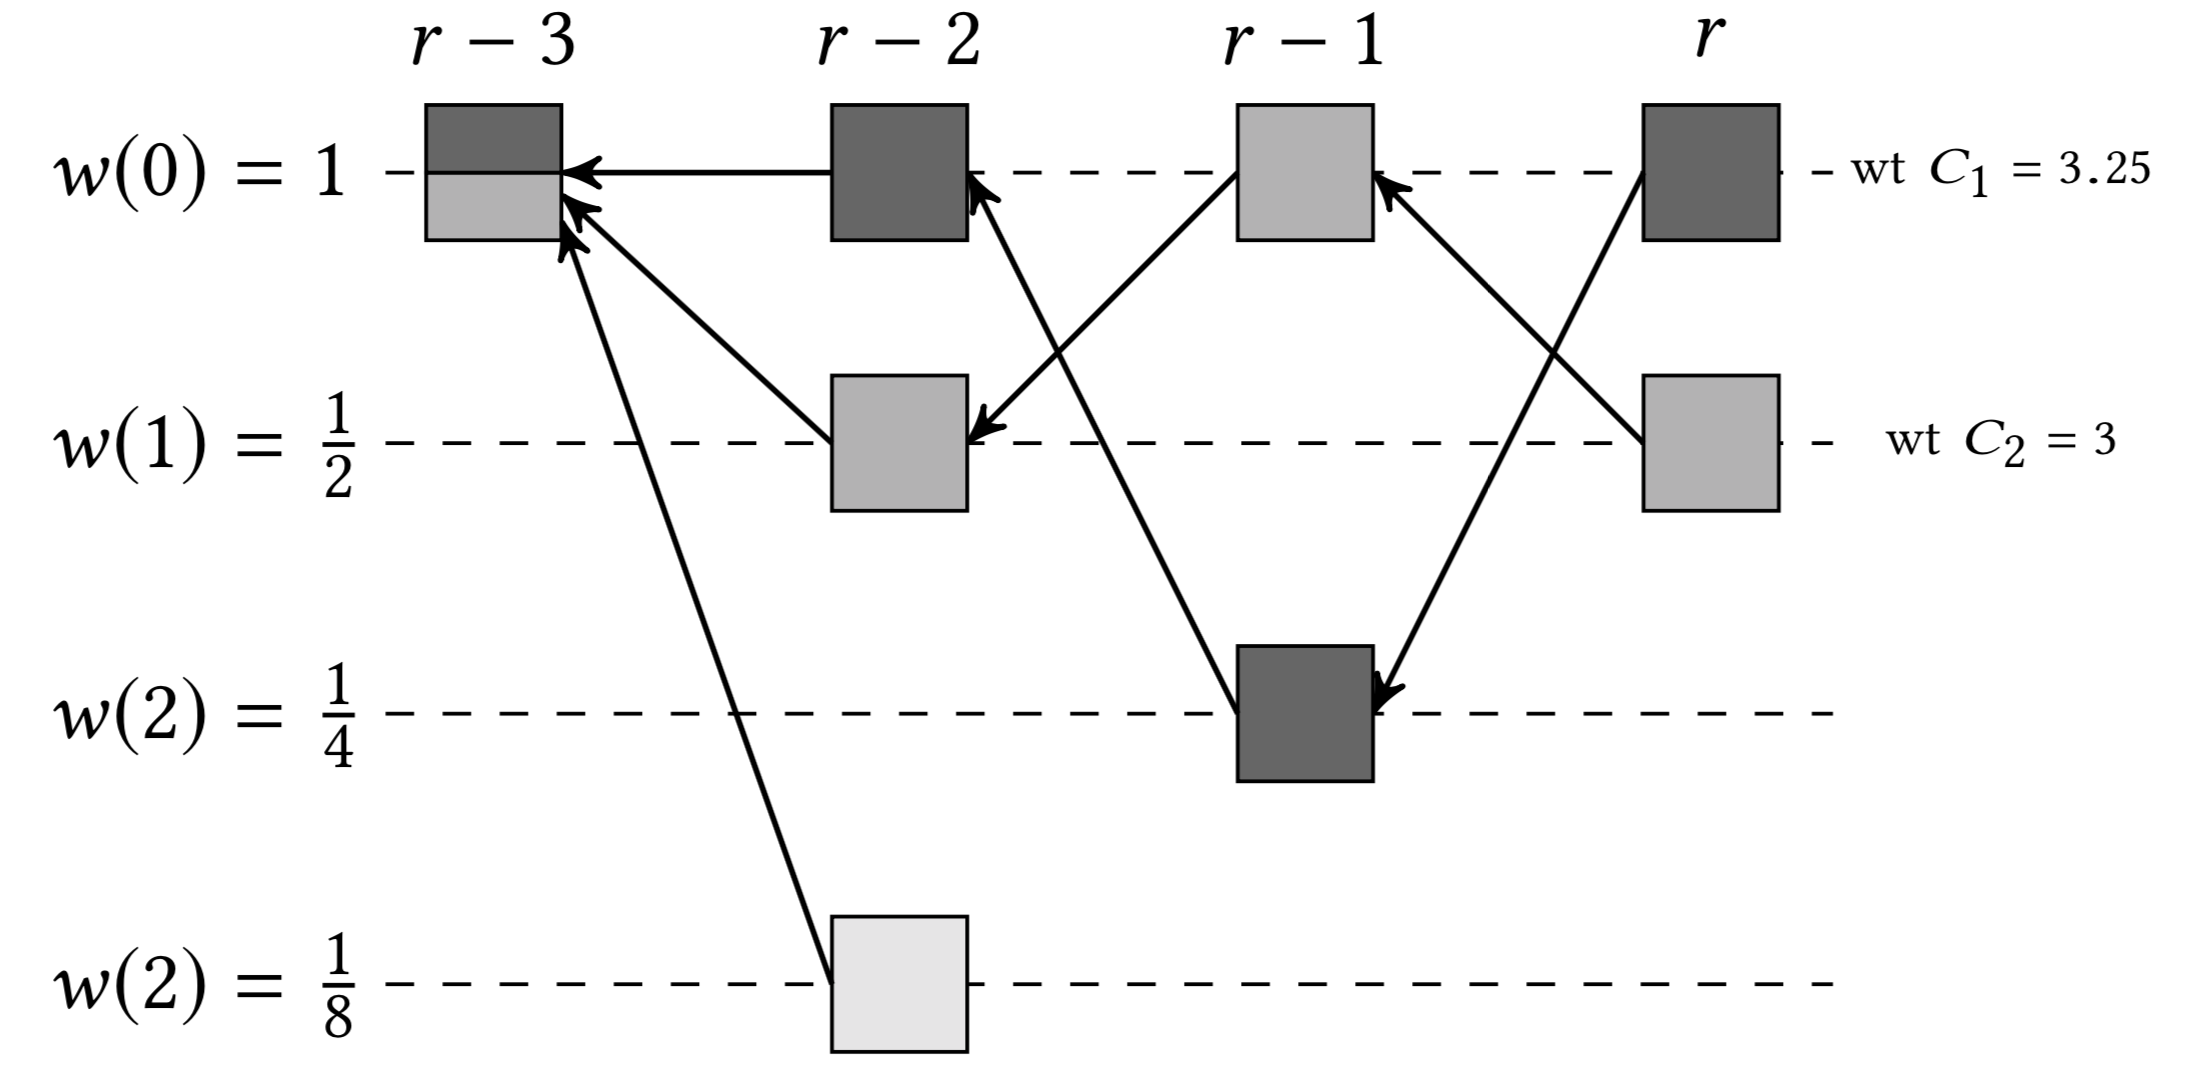
\includegraphics[width=0.8\textwidth]{../common/Dfinity_1.png}
	\caption{Dfinity区块链权重举例。四条横轴虚线对应四个矿工且权重分别为$1,1/2,1/4,1/8$。图中区块不同深浅对应与该区块属于哪一条区块链(共3条,$C_1$颜色最深,$C_3$颜色最浅)。通过计算表明链$C_1$拥有最高的总权重} 		
	\label{fig:Dfinity1}
\end{figure}
\textbf{区块提出}
矿工将区块接到权重最高的链上。注意,公证层被公证的区块仍是当前轮排名最高的区块。同时将新区块进行广播以请求公证。

\textbf{区块公证}
首先Dfinity的公证是每轮进行的。如果区块被揭露得过晚则永远不会被公证。这样有效的防止了私自挖矿(selfish mining)进攻。

一个区块被公证了当且仅当它收到了大部分公证者的签名。对每个公证者(委员会成员,也是客户端或副本节点replica),具体的公证算法用文字描述如下:
\begin{itemize}
	\item 设当前轮数为$r$。等待Blocktime时间
	\item 如果没有收到任何被公证的区块,则选择第$r$轮接收到的所有区块中排名最高的一个,对其进行签名并广播。
	\item 如果收到了被公证的区块,则$r=r+1$
\end{itemize}
文章把当前轮只有一个区块被公证的情况称作常规操作(normal operation),然后针对常规操作分析了确认时间及安全性等,但这本身是一个比较强的假设。

\textbf{最终确认}
之所以公证化不等于最终确认,是因为因传输延迟等影响存在多个区块被公证的情况。这是还需要一个最终确认(finalize)算法。

该算法描述如下:在第$r$轮,节点等待$T$时刻以接受第$r$轮被公证的区块并放入集合$N_{r}$,随后执行$Finalize(r-1)$,即,把$N_{r-1}$(即,第$r-1$轮被公正的区块集)的最长公共前缀标为最终确认。\reffig{fig:Dfinity2}指出了最终确认的过程。

同时需要基于假设:在$Finalize(h)$被执行时,$N_h$包含第$h$轮所有被公证的区块。

关于最终确认的主要定理为,在常规操作下任何交易都会在接收到两个确认信息后(被公证区块$B_r$打包,同时区块$B_{r+1}$接在上面)加上网络延迟时间的两倍内被最终确认。

\begin{figure}
	\centering
	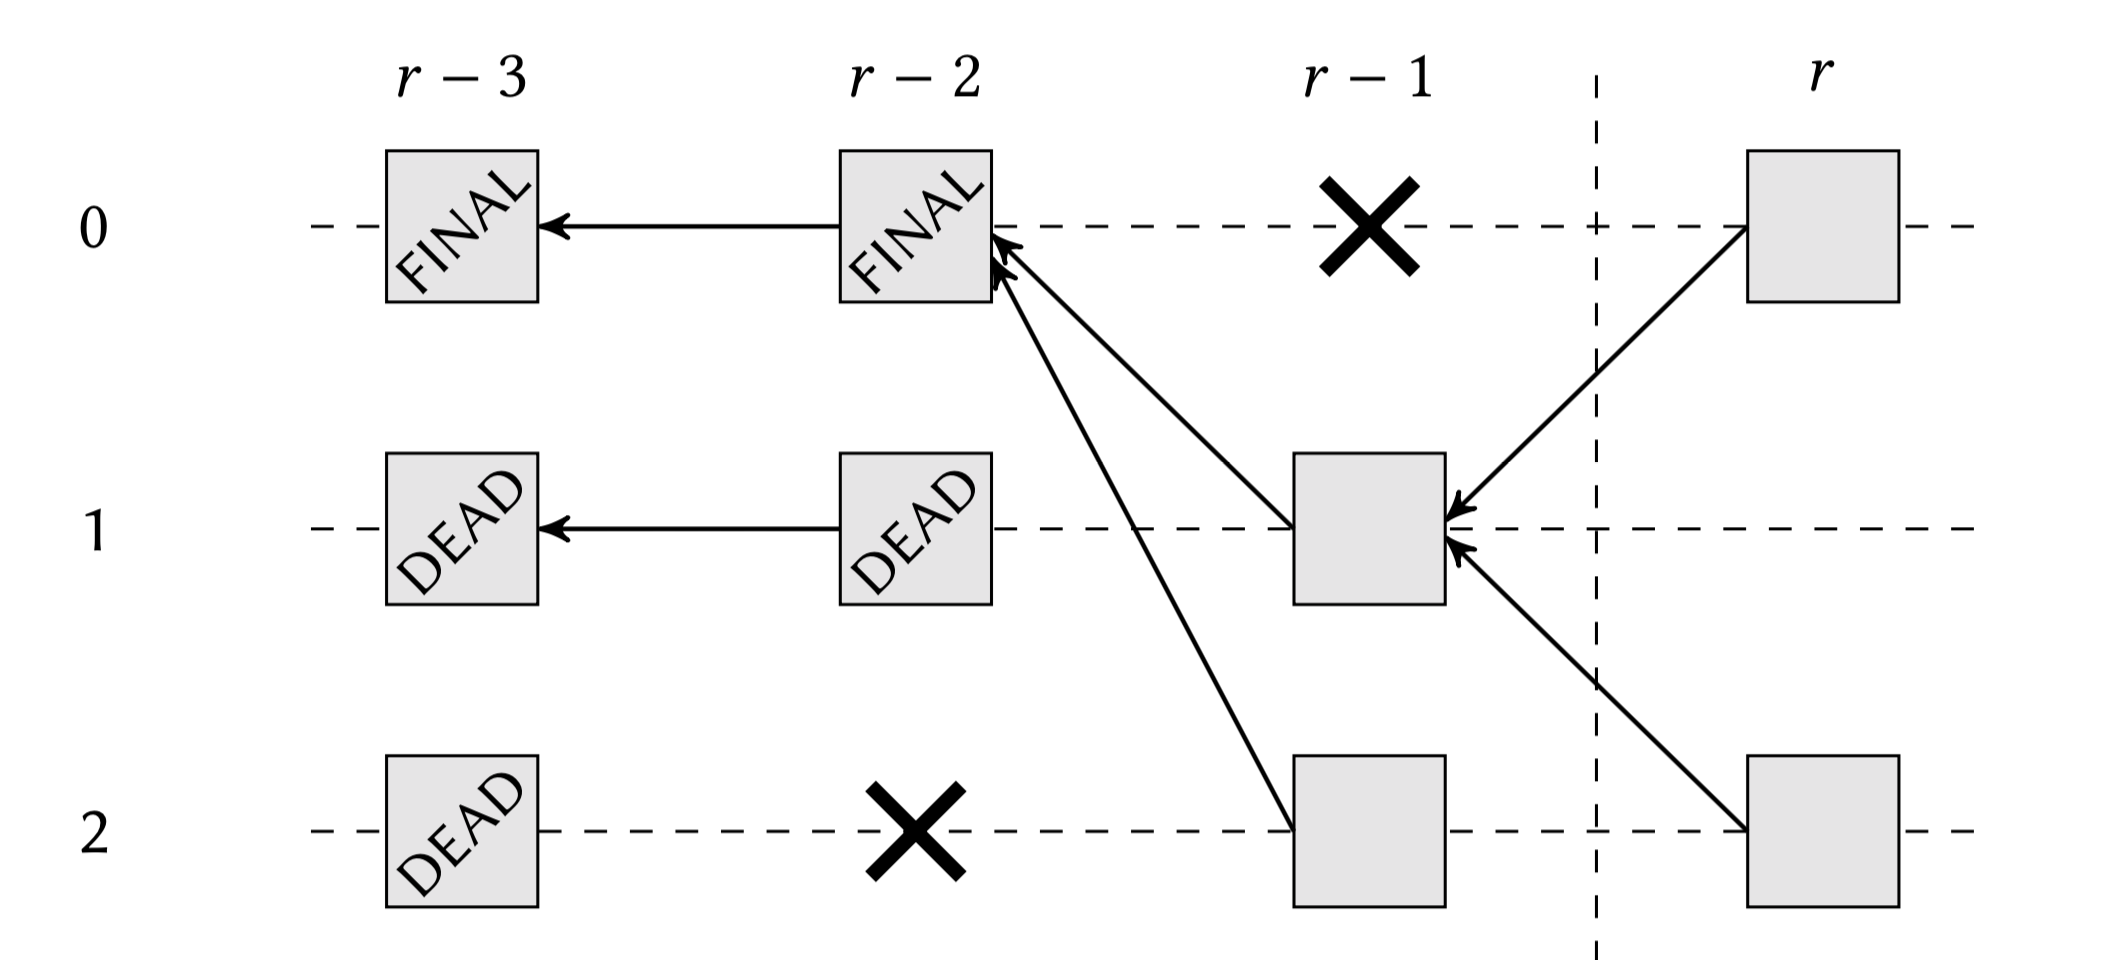
\includegraphics[width=0.8\textwidth]{../common/Dfinity_2.png}
	\caption{Dfinity区块最终确认。第$r$轮加$T$时间执行第$r-1$轮的最终确认。} 		
	\label{fig:Dfinity2}
\end{figure}

\subsection{门限签名}
关于具体原理涉及到密码学的诸多知识,这里不多做介绍。这里说明的是,$t,n$门限签名实现的主要功能为,一旦获得了$n$个人中$t$个人的签名$\sigma_{i_1},...,\sigma_{i_t}$,则可以算出所需的组签名$\sigma$。该组签名可以被任何人验证(组公钥为公开信息),且所有人的私钥仍没有被透露。其工作原理大致是用的是$t-1$次多项式函数可以被$t$个点唯一确定。

Dfinity随机种子层的工作原理就是用的门限签名。在第$r$轮开始是,每个委员会成员计算签名
$$\sigma_{r,i}=Sign(r||\xi_{r-1},sk_{G,i})$$
其中$sk_{G,i}$为成员$i$在委员会$G$中的私钥。

随后,根据$t$个签名$\sigma_{r,i}$计算出组签名$\sigma_r$,将其哈希值作为第$r$轮的输出$\xi_r$。

该签名方案简单实用,事实上被绝大部分区块链项目所使用。

Dfinity最后还提到了朝代(epoch)的概念,朝代更迭是开展对客户端/委员会候补集合的申请与注销工作。
\subsection{总结与思考}
关于VRF的使用,不可预测性和可验证性都是必须要满足的条件。其中不可预测性就意味着随机种子不能是固定值。所以,随机种子的选取非常重要,在没有全局时钟的情况下,由前一个区块的数据及当前区块高度共同决定是可行的方案。Dfinity对VRF的应用和投票思想都很清晰严谨,具有很高的借鉴意义。事实上,TAS chain白皮书\footnote{https://www.taschain.io/static/pdf/TASChainTechnologyWhitePaper.pdf}大部分就是借鉴Dfinity。不足之处在于假设过多,真正的安全性和性能存疑,而且准入门槛对于permissionless的公链也是个难以解决的问题。
